\section{Método}
\begin{frame}{Método}{}
    \begin{itemize}
        \item Algoritmo de Krumhansl-Schmukler
        \item Key Profiles
        \begin{itemize}
            \item Krumhansl
            \item Variações: Temperley / Aarden / Bellman / Simple (Craig)
        \end{itemize}
        \item Exemplo
    \end{itemize}
\end{frame}

\subsection{Algoritmo de Krumhansl-Schmukler}
\begin{frame}{Método}{Algoritmo de Krumhansl-Schmukler}
    \begin{columns}[]
        \begin{column}{.5\textwidth}
            \begin{itemize}
                \item Baseado em perfis tonais (\textit{Key Profiles})
                \item Construção de uma distruibuição representativa da presença de cada nota
                \begin{itemize}
                    \item Temporal e variável com a métrica escolhida
                \end{itemize}
                \item Autocorrelação com cada perfil tonal
                \begin{itemize}
                    \item Perfil com maior correlação é o escolhido
                \end{itemize}
            \end{itemize}
        \end{column}
        \begin{column}{.5\textwidth}
            \begin{figure}
                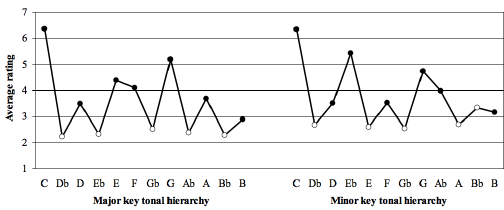
\includegraphics[width=.9\textwidth]{figs/key_profiles_C.png}
            \end{figure}
        \end{column}
    \end{columns}
\end{frame}

\subsection{Key Profiles}
\begin{frame}{Método}{Key Profiles}
    \begin{itemize}
        \item Krumhansl-Schmukler \& Kessler
        \begin{itemize}
            \item Análise subjetiva com voluntários 
            \item Quão bem uma nota soa num elemento musical de uma tonalidade (Escala, Cadência, etc)
            \item Contrução de um perfil tonal para todas as tonalidades maiores e outra para as menores
        \end{itemize}
        \item Temperley
        \item Bellman e Aarden
        \item Simple (Craig)
    \end{itemize}
\end{frame}

\subsection{Exemplo}
\begin{frame}{Método}{Exemplo}
    \begin{columns}[]
        \begin{column}{.5\textwidth}
            \begin{itemize}
                \item Melodia "Yankee Doodle"
                \item Construção da distruibuição
                \item Correlação com os perfis de Krumhansl
                \item Melhor previsão - G Major (0.693)
                \begin{itemize}
                    \item D Major (0.485)
                    \item E Minor (0.398)
                    \item G Minor (0.394)
                \end{itemize}
            \end{itemize}
        \end{column}
        \begin{column}{.5\textwidth}
            \begin{figure}
                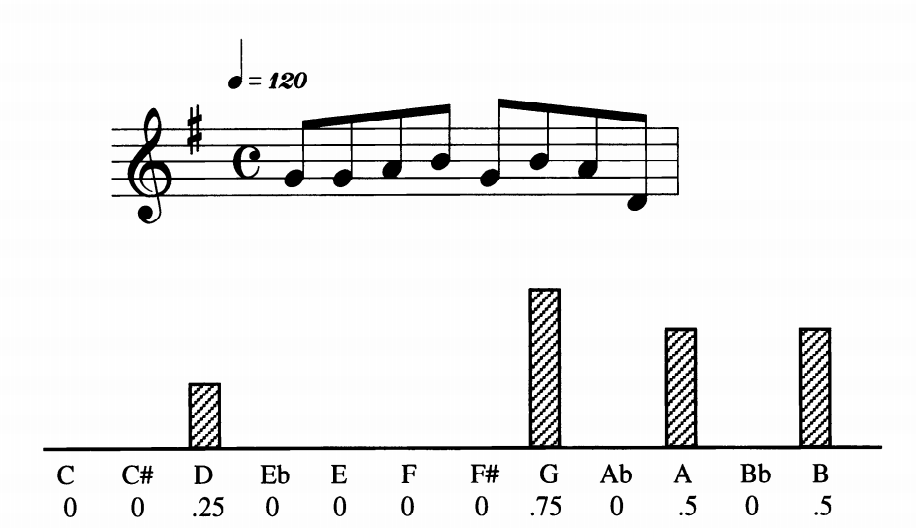
\includegraphics[width=.9\textwidth]{figs/yankee_song.png}
            \end{figure}
        \end{column}
    \end{columns}
\end{frame}